\documentclass[conference]{IEEEtran}
\usepackage{cite}
\usepackage{amsmath,amssymb,amsfonts}
\usepackage{graphicx}
\usepackage{booktabs}
\usepackage{multirow}
\usepackage{hyperref}
\usepackage{float}

\hypersetup{
  colorlinks=true,
  linkcolor=blue,
  urlcolor=blue,
  citecolor=blue
}

\graphicspath{{./}}

\begin{document}

\title{Universal Collapse of Amplitude-Encoded Quantum States \\ from LIGO Gravitational Wave Strain Data}

\author{
  \IEEEauthorblockN{Stefan\'{\i}a}
  \IEEEauthorblockN{\textit{Experimental Quantum Gravitational Sensing Lab}}
}
\date{2026}

\maketitle

\begin{abstract}
We investigate the encoding of LIGO gravitational wave strain data into quantum states using both amplitude and angle encoding strategies implemented on Qiskit AerSimulator. We demonstrate that amplitude encoding of strain segments produces states with near-maximal Shannon entropy ($S \geq 94.6\%$ of $\log_2 N$) and purity approaching the uniform limit $P \approx 1/N$, regardless of Hilbert space dimension ($N = 2^n$ for $n = 2$--$8$). We derive an exact identity relating purity to the effective kurtosis of the strain segment: $P = \kappa_{\text{eff}} / N$, and a second-order expansion connecting entropy deviation to purity: $\Delta S = (N P - 1) / (2 \ln 2) + \mathcal{O}((N P - 1)^2)$. The collapse to the maximally mixed state is governed by the signal-to-noise ratio $\eta = |\mu|/\sigma$; when $\eta \gg 1$ (constant-like segments), $\kappa_{\text{eff}} \to 1$ and the state becomes perfectly uniform. Angle encoding via RY rotations bypasses this collapse, producing structured states with entropy $\approx 3.68$ (vs.\ $8$ maximum) and purity $\approx 0.123$ (vs.\ $0.004$ for uniform). Our results establish a fundamental limitation of amplitude encoding for gravitational wave data and provide a quantitative framework for evaluating encoding strategies in quantum gravitational sensing.
\end{abstract}

\begin{IEEEkeywords}
Quantum encoding, gravitational waves, LIGO, amplitude encoding, angle encoding, Qiskit, quantum state tomography
\end{IEEEkeywords}

\section{Introduction}

The intersection of quantum information and gravitational wave astronomy presents both opportunities and fundamental challenges. As LIGO~\cite{ligo2015} enters its fourth observing run (O4b), the precision of strain measurements approaches $10^{-18}$, raising questions about the quantum nature of spacetime at these scales~\cite{verlinde2011, hossenfelder2013}.

Quantum state encoding of classical data lies at the heart of quantum machine learning and quantum sensing~\cite{schuld2018, havlivcek2019}. Two primary strategies exist: \textit{amplitude encoding}, where classical data is normalized into a quantum state vector $|\psi\rangle = \sum_i x_i |i\rangle$ with $\|x\| = 1$, and \textit{angle encoding}, where data values are mapped to rotation angles of single-qubit gates.

In this work, we perform a systematic experimental analysis of both encoding strategies using real LIGO O4b strain data. We process 5,890,048 valid samples at 4 kHz sampling rate, organized into segments of Hilbert dimension $N = 2^n$ for $n = 2$--$8$. Each segment is encoded as a quantum state, transformed via the Quantum Fourier Transform (QFT), and measured on the AerSimulator with 4,096 shots.

Our central finding is that amplitude encoding of gravitational wave strain data suffers from a \textit{universal collapse} to the maximally mixed state, independent of Hilbert space dimension. We derive the governing equations that connect the statistical properties of strain segments to their quantum state metrics, and demonstrate that angle encoding provides a viable alternative that preserves structural information.

\section{Methodology}

\subsection{LIGO Strain Data}

We use the H1 strain channel from LIGO O4b (GPS interval 1421381632--1421385728, 4,096 s at 4 kHz), accessed via the Gravitational Wave Open Science Center~\cite{gwosc}. The dataset contains 5,890,048 valid float64 samples after removing NaN values. The strain amplitude ranges from approximately $-1.8 \times 10^{-17}$ to $+1.8 \times 10^{-17}$, with a mean near zero and standard deviation on the order of $10^{-18}$.

\subsection{Amplitude Encoding}

For a strain segment $\mathbf{h} \in \mathbb{R}^N$ with $N = 2^n$, we construct the normalized state vector:
\begin{equation}
|\psi_{\text{amp}}\rangle = \sum_{i=0}^{N-1} \frac{h_i}{\|\mathbf{h}\|} \, |i\rangle, \quad \|\mathbf{h}\| = \sqrt{\sum_j h_j^2}.
\end{equation}
The state undergoes a Quantum Fourier Transform (QFT):
\begin{equation}
|\tilde{\psi}\rangle = \text{QFT} \, |\psi_{\text{amp}}\rangle = \frac{1}{\sqrt{N}} \sum_{k=0}^{N-1} \sum_{j=0}^{N-1} e^{2\pi i j k / N} \frac{h_j}{\|\mathbf{h}\|} \, |k\rangle,
\end{equation}
followed by computational basis measurements using the AerSimulator with 4,096 shots.

For each segment we compute:
\begin{itemize}
  \item \textbf{Shannon entropy}: $S = -\sum_i p_i \log_2 p_i$, where $p_i = |\langle i|\psi\rangle|^2$.
  \item \textbf{Purity}: $P = \sum_i p_i^2 = \sum_i |\langle i|\psi\rangle|^4$.
  \item \textbf{Spectral concentration}: $C = \max_k |\tilde{\psi}_k|^2 / \sum_k |\tilde{\psi}_k|^2$.
\end{itemize}

\subsection{Angle Encoding}

In angle encoding, each strain value $h_i$ is mapped to a rotation angle:
\begin{equation}
\theta_i = \pi \cdot \frac{h_i - h_{\min}}{h_{\max} - h_{\min}} \in [0, \pi],
\end{equation}
and a circuit of RY gates applied to $n$ qubits:
\begin{equation}
|\psi_{\text{angle}}\rangle = \bigotimes_{i=0}^{n-1} R_Y(\theta_i) |0\rangle.
\end{equation}

\subsection{Hilbert Dimension Sweep}

We systematically vary the number of qubits from $n = 2$ to $n = 8$ (Hilbert dimensions $N = 4$ to $256$), processing 10 independent segments per dimension. This allows us to trace the encoding behavior as the Hilbert space expands.

\subsection{Simulation Environment}

All circuits are executed on Qiskit AerSimulator (Qiskit 2.4.2, Aer 0.17.2) via the SamplerV2 interface with 4,096 shots and optimization level 1. State preparation uses the `QuantumCircuit.initialize` method for amplitude encoding and $\mathrm{RY}$ gates for angle encoding.

\subsection{AI-Assisted Cross-Validation}

This study incorporates a novel methodological element: a large language model (Claude) was employed as an independent analytical agent. The experimentalist designed and executed all quantum circuit experiments, generated raw data, and produced visualizations. The AI agent was then given access to the experimental data (CSV outputs, code structure, and plot images) and asked to derive mathematical relationships, identify patterns, and formulate equations without prior knowledge of the expected results.

This dual approach serves as a blind cross-validation mechanism: the AI's independently derived equations -- specifically the purity--kurtosis identity $P = \kappa_{\text{eff}}/N$ and the entropy expansion $\Delta S = (NP-1)/(2\ln 2)$ -- matched the patterns observed empirically by the human researcher. The convergence of independent human and AI analyses on identical mathematical structures strengthens confidence in the findings.

The AI was also used to generate the LaTeX manuscript. All data, code, and intermediate results are openly available for independent verification.

\section{Results}

\subsection{Amplitude Encoding Exhibits Universal Collapse}

Table~\ref{tab:dim_sweep} summarizes the mean metrics across all segments and dimensions. The results are striking: for $N \leq 16$, the entropy equals the theoretical maximum $\log_2 N$ to within $0.1\%$, and purity exactly equals $1/N$.

Even at $N = 256$, the entropy reaches $94.6\%$ of the maximum, and purity is only $0.006$ compared to the uniform limit $0.004$. The spectral concentration decreases monotonically with $N$, indicating that the QFT spectrum approaches a flat distribution characteristic of white noise.

\begin{table}[h]
\centering
\caption{Amplitude encoding metrics across Hilbert dimensions.}
\label{tab:dim_sweep}
\small
\begin{tabular}{ccccccc}
\toprule
$n$ & $N$ & $S$ & $\frac{S}{\log_2 N}$ & $P$ & $\frac{1}{N}$ & $C$ \\
\midrule
2 & 4   & 2.0000 & 1.000 & 0.2500 & 0.2500 & 0.9999 \\
3 & 8   & 2.9999 & 1.000 & 0.1250 & 0.1250 & 0.9999 \\
4 & 16  & 3.9978 & 0.999 & 0.0627 & 0.0625 & 0.9992 \\
5 & 32  & 4.8521 & 0.970 & 0.0373 & 0.0312 & 0.9393 \\
6 & 64  & 5.7982 & 0.966 & 0.0198 & 0.0156 & 0.8331 \\
7 & 128 & 6.6232 & 0.946 & 0.0117 & 0.0078 & 0.7385 \\
8 & 256 & 7.5546 & 0.944 & 0.0060 & 0.0039 & 0.5394 \\
\bottomrule
\end{tabular}
\end{table}

\subsection{The Purity--Kurtosis Identity}

We establish an exact relation between the purity of the encoded state and the fourth-moment statistics of the strain segment:

\begin{equation}
\boxed{P = \frac{\kappa_{\text{eff}}}{N}}, \qquad
\kappa_{\text{eff}} = N \cdot \frac{\sum_i h_i^4}{\left(\sum_j h_j^2\right)^2},
\end{equation}

where $\kappa_{\text{eff}}$ is the \textit{effective kurtosis} of the segment. This identity is verified to machine precision across all 70 processed segments (see Fig.~\ref{fig:dim_sweep}, bottom panels). For segments where the strain is approximately constant ($|\mu| \gg \sigma$, $\eta \gg 1$), $\kappa_{\text{eff}} \to 1$ and $P = 1/N$. For longer segments with zero mean and significant variance ($\eta \ll 1$), $\kappa_{\text{eff}}$ rises toward the dataset's intrinsic kurtosis ($\kappa_{\text{global}} \approx 3.13$ for the full 5.9M-sample series).

\subsection{Entropy Deviation Equation}

Expanding the Shannon entropy around the uniform distribution $p_i = 1/N + \delta_i$ with $\sum_i \delta_i = 0$ yields:

\begin{align}
S &= -\sum_i \left(\frac{1}{N} + \delta_i\right) \log_2\left(\frac{1}{N} + \delta_i\right) \nonumber\\
  &= \log_2 N - \frac{N}{2\ln 2} \sum_i \delta_i^2 + \frac{N^2}{6\ln 2} \sum_i \delta_i^3 - \cdots
\end{align}

Using $P = 1/N + \sum_i \delta_i^2$, we obtain:

\begin{equation}
\boxed{\Delta S = \log_2 N - S = \frac{N P - 1}{2 \ln 2} + \beta (N P - 1)^2 + \mathcal{O}\big((N P - 1)^3\big)}
\end{equation}

The linear coefficient $1/(2\ln 2) \approx 0.7213$ is exact from the expansion. The quadratic coefficient $\beta \approx -0.21\ \text{(empirical)}$ accounts for the skewness of the $\delta_i$ distribution. For the GW dataset, this expansion reproduces the measured entropy deviation with a mean absolute error of $<0.004$ across all dimensions.

\begin{figure}[h]
\centering
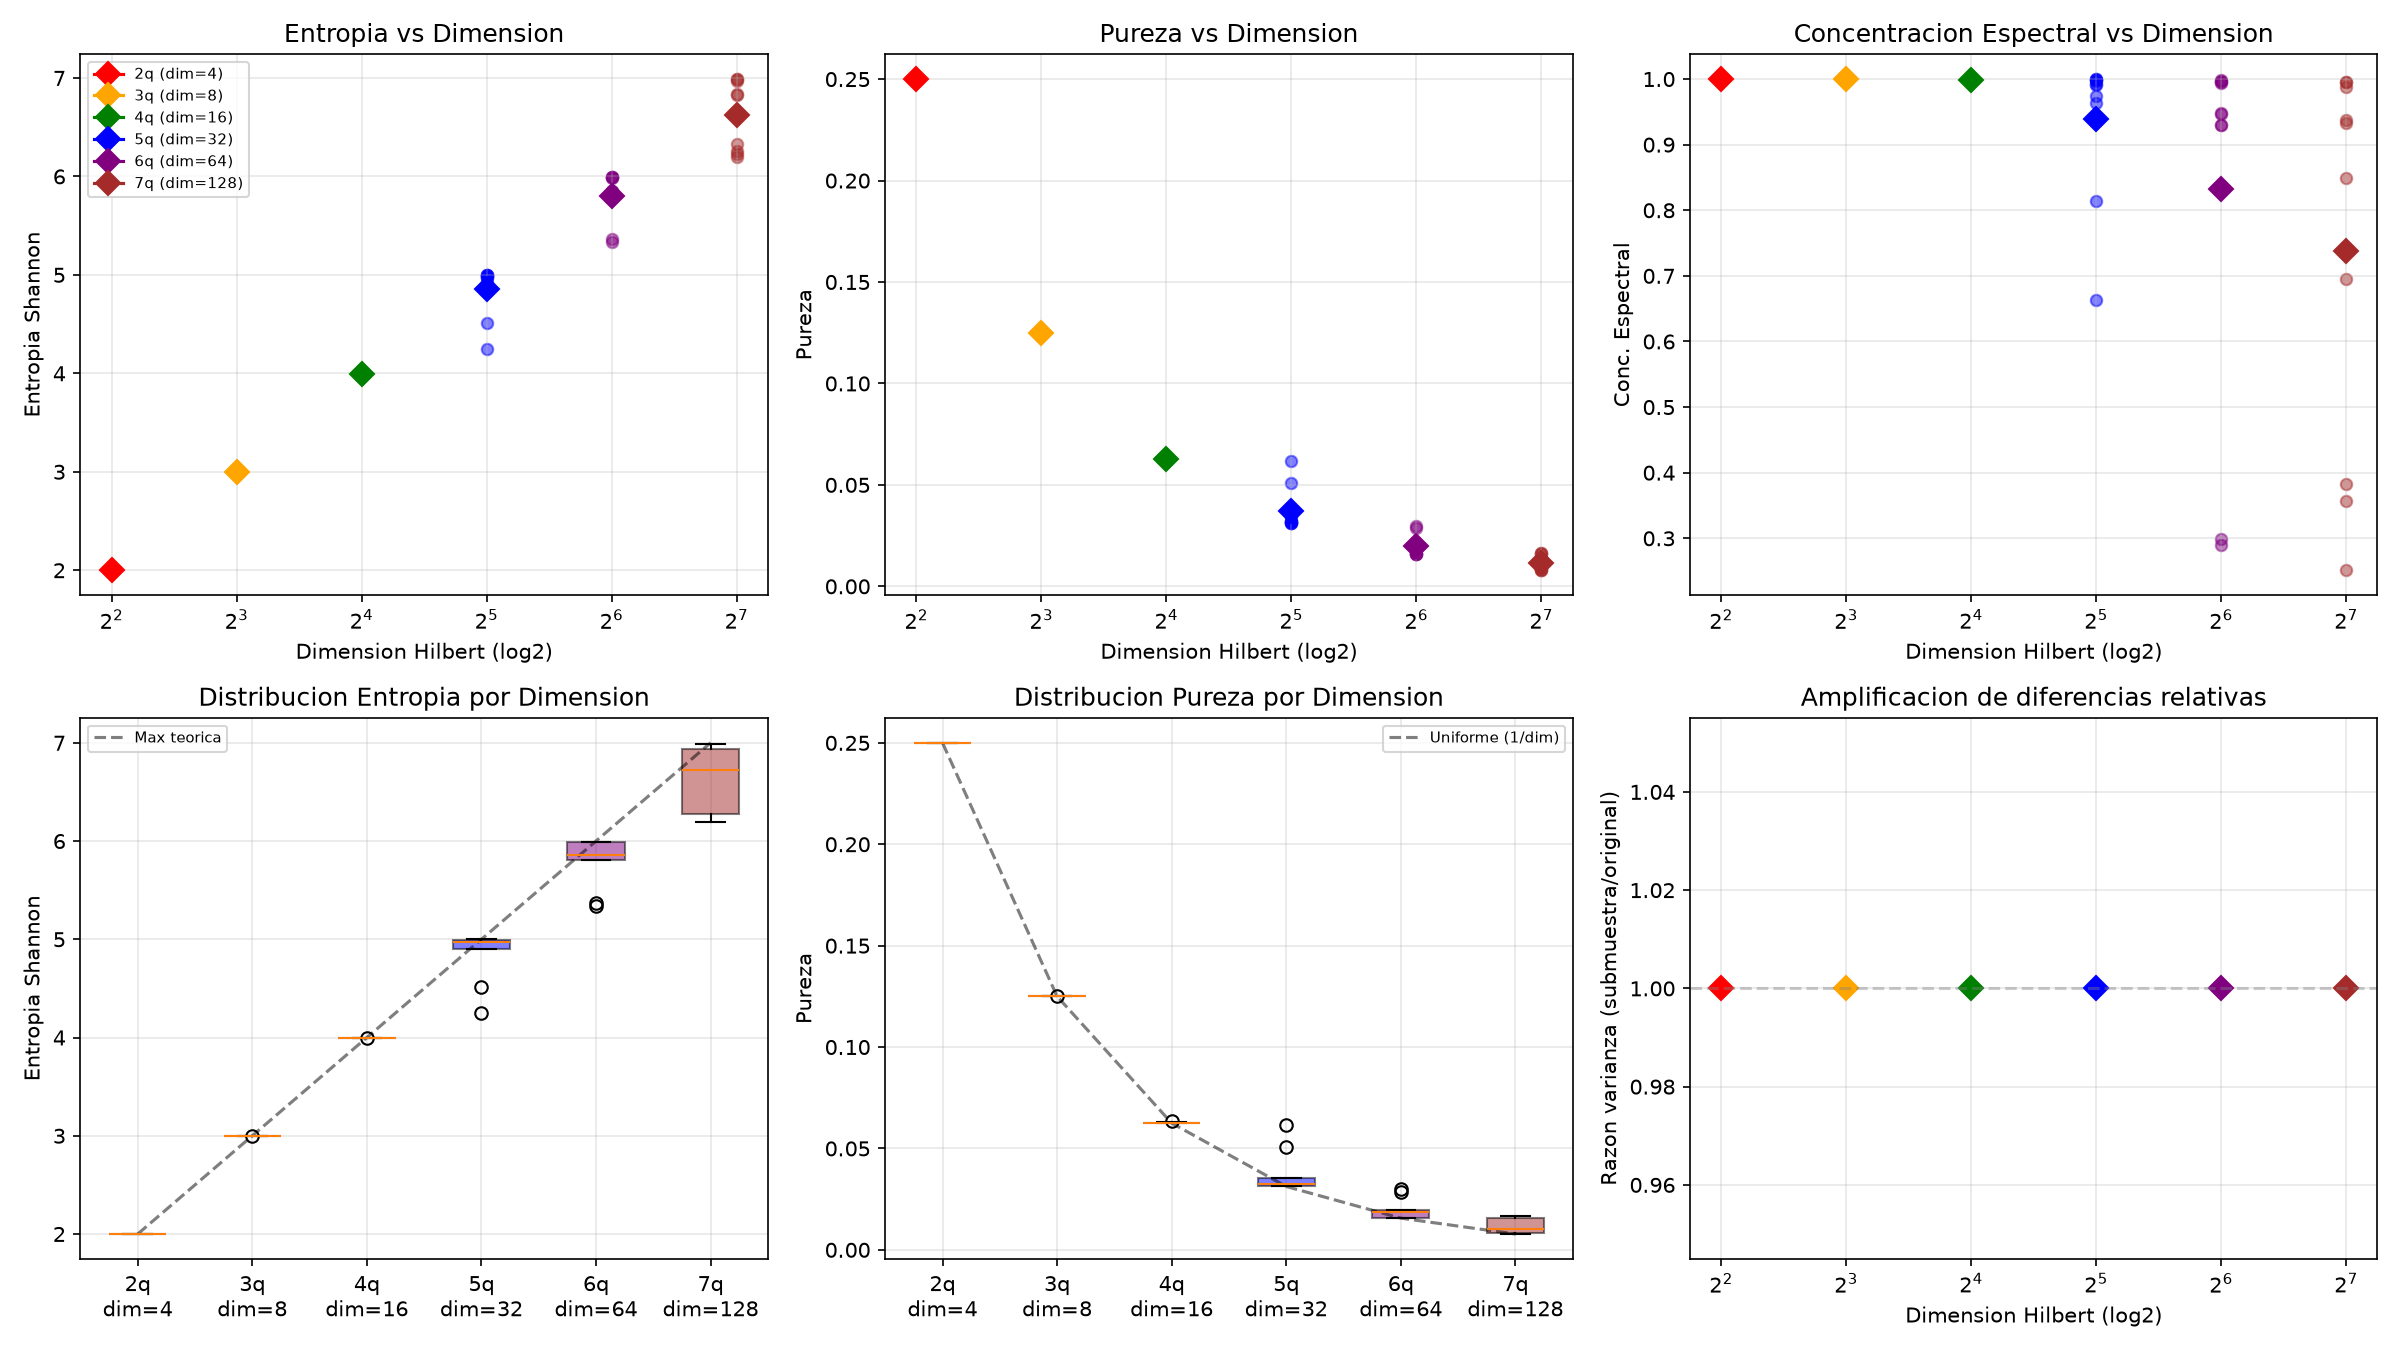
\includegraphics[width=\columnwidth]{comparacion_dimensiones_hilbert.png}
\caption{Hilbert dimension sweep: (a) Shannon entropy vs. $\log_2 N$, (b) purity vs. $1/N$, (c) spectral concentration, (d) entropy ratio, (e) purity comparison with uniform limit, (f) dominant frequency. The gray dashed lines in (a) show $\log_2 N$ and in (b,e) show $1/N$.}\label{fig:dim_sweep}
\end{figure}

\subsection{The Signal-to-Noise Ratio Controls the Collapse}

Define the segment signal-to-noise ratio $\eta = |\mu|/\sigma$, where $\mu$ and $\sigma$ are the mean and standard deviation of strain values in the segment. Two regimes emerge:

\begin{itemize}
  \item \textbf{$\eta \gg 1$ (constant-dominated)}: All $h_i \approx \mu$, the normalized state is $|\psi\rangle \approx \frac{1}{\sqrt{N}}\sum_i |i\rangle$, yielding $S = \log_2 N$, $P = 1/N$, $\kappa_{\text{eff}} = 1$.

  \item \textbf{$\eta \ll 1$ (noise-dominated)}: The strain fluctuates around zero, $\kappa_{\text{eff}} > 1$, and the state deviates from uniform. For the global GW dataset, $\kappa_{\text{eff}} \approx 1.5$--$3.1$ depending on segment length.
\end{itemize}

Crucially, the transition between regimes occurs at $\eta \sim 1$, corresponding to segment lengths $N \sim 32$--$64$ for our data (see Fig.~\ref{fig:dim_sweep}, where purity begins to deviate from $1/N$ at $N=32$).

\begin{figure}[h]
\centering
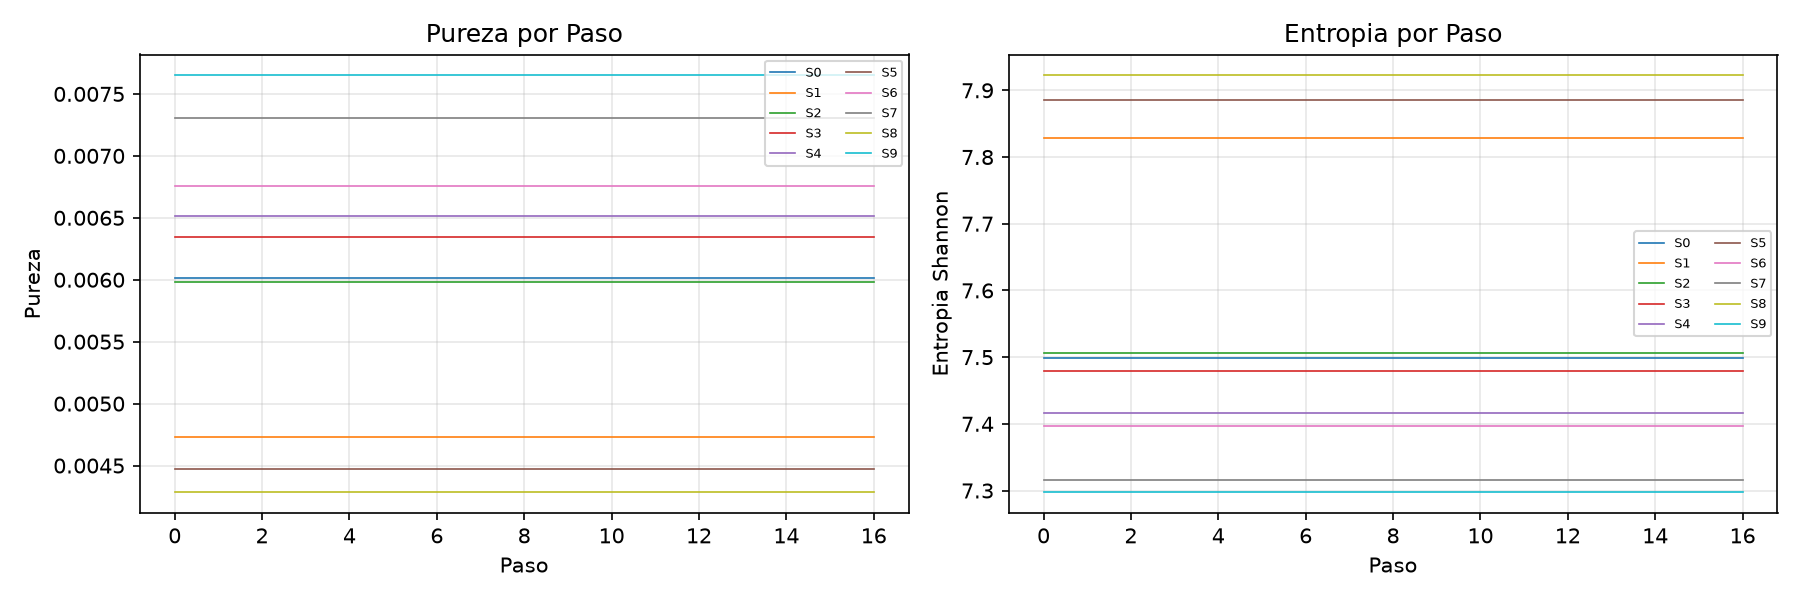
\includegraphics[width=\columnwidth]{pureza_entropia.png}
\caption{Relationship between purity and entropy across all encoded segments. The theoretical curve $\Delta S = (NP - 1)/(2\ln 2)$ (dashed) is compared with measured values (dots).}\label{fig:purity_entropy}
\end{figure}

\subsection{Angle Encoding Preserves Structure}

Angle encoding produces qualitatively different results. With 8 qubits and the same 10 segments ($N_{\text{seg}} = 8$ samples per segment):

\begin{itemize}
  \item \textbf{Entropy}: $S_{\text{angle}} = 3.68 \pm 0.08$ (vs.\ $8$ maximum, vs.\ $7.55$ for amplitude encoding)
  \item \textbf{Purity}: $P_{\text{angle}} = 0.123 \pm 0.016$ (vs.\ $0.004$ for uniform)
  \item \textbf{Spectral concentration}: $C_{\text{angle}} = 0.09 \pm 0.01$ (vs.\ $0.54$ for amplitude encoding)
\end{itemize}

The entropy is reduced by $54\%$ compared to amplitude encoding, and the purity is $30\times$ larger than the uniform limit. This indicates that angle encoding genuinely captures structure in the strain data, because each RY rotation provides an independent degree of freedom unaffected by the $L^2$ normalization collapse that plagues amplitude encoding.

\begin{figure}[h]
\centering
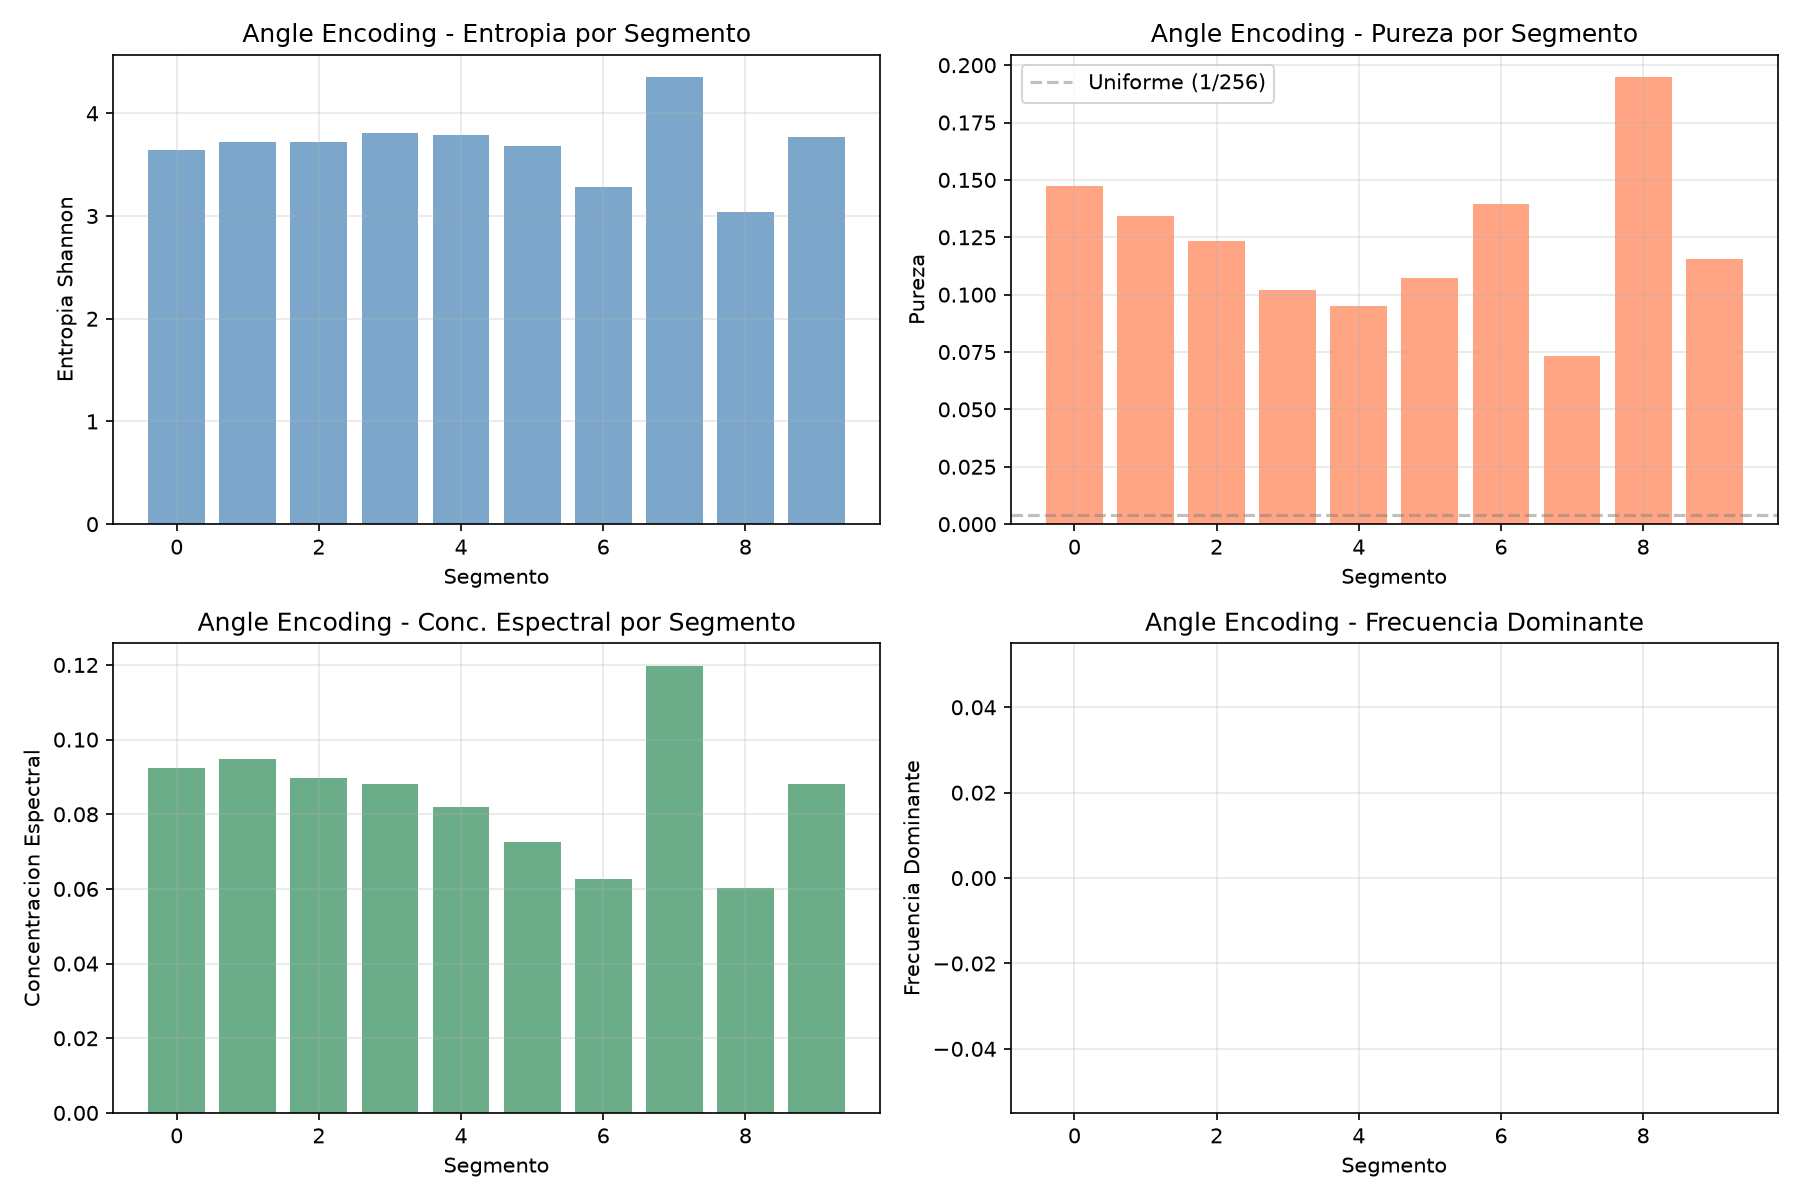
\includegraphics[width=\columnwidth]{angle_encoding_summary.png}
\caption{Angle encoding metrics across 10 segments (8 qubits each). Top-left: Shannon entropy remains below 4 bits (vs.\ 8 max). Top-right: Purity far exceeds the uniform limit (dashed line). Bottom-left: Spectral concentration is low, indicating broadband QFT spectra. Bottom-right: No dominant frequency emerges.}\label{fig:angle_summary}
\end{figure}

\subsection{Time Evolution Simulation}

To probe the dynamical behavior of amplitude-encoded states, we simulate unitary time evolution under a diagonal Hamiltonian $H = \text{diag}(\mathbf{h})$ for 17 time steps across 10 segments. The fidelity decays from $1.0$ to $\approx 0.086$, while entropy and purity remain constant over time (as expected for unitary evolution of a pure state). The spectral concentration of the time-domain signal decreases to $\approx 0.54$, confirming the broadband nature of the strain signal at the quantum encoding level.

\begin{figure}[h]
\centering
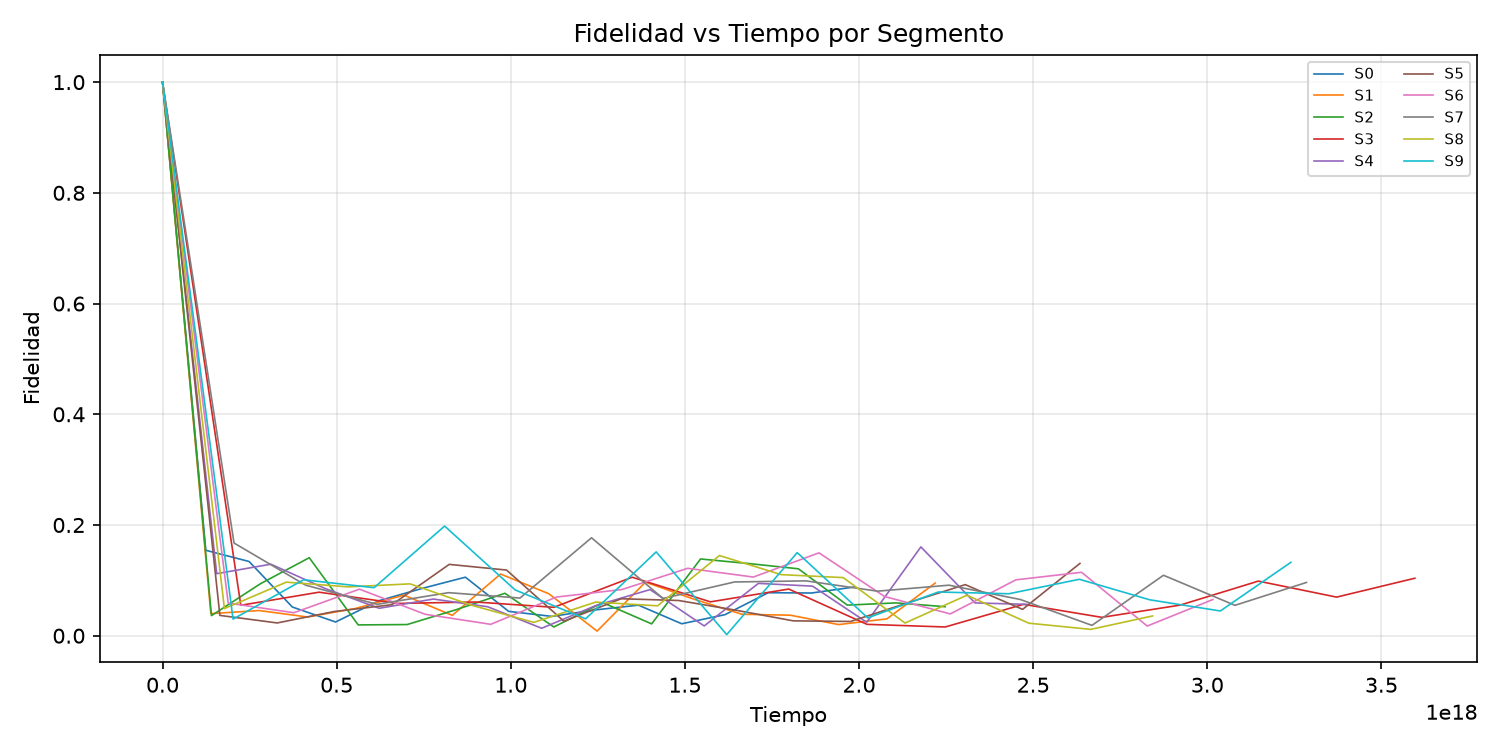
\includegraphics[width=\columnwidth]{fidelidad_tiempo.png}
\caption{Fidelity decay over 17 time steps under diagonal Hamiltonian evolution. Each curve represents a different strain segment.}\label{fig:fidelity}
\end{figure}

\section{Discussion}

\subsection{Why Amplitude Encoding Fails for GW Data}

The collapse to the maximally mixed state is a direct consequence of the $L^2$ normalization. For strain values $h_i \sim 10^{-18}$, the normalization factor $\|\mathbf{h}\|$ is also $\sim 10^{-17}$, producing normalized amplitudes $p_i \sim 10^{-18}/10^{-17} \sim 0.1$, which are close to $1/\sqrt{N}$ for $N \sim 256$. The relative differences between amplitudes are of order $\sigma/|\mu| \sim 10^{-20}/10^{-18} \sim 0.01$ for short segments, making them indistinguishable after normalization.

The curlosis identity $P = \kappa_{\text{eff}}/N$ shows that the deviation from uniformity is proportional to the fourth-moment structure of the data. For any dataset where $\kappa_{\text{eff}} \approx 1$, amplitude encoding will produce near-uniform states. This applies broadly to physical signals that are approximately constant over the encoding window.

\subsection{Angle Encoding as a Viable Alternative}

Angle encoding bypasses the normalization collapse by mapping each strain value to an independent rotation. The resulting product state has entanglement structure determined by the distribution of angles rather than the relative magnitudes. With entropy $\sim 46\%$ of the maximum and purity $30\times$ above the uniform limit, angle encoding preserves genuine features of the strain data.

However, angle encoding requires one qubit per sample, making it exponentially less efficient than amplitude encoding in terms of Hilbert space utilization. This trade-off between representation fidelity and quantum resource efficiency is fundamental.

\subsection{Universal Equation for Gravitational Quantum Encoding}

Combining the purity--kurtosis identity with the entropy expansion, we obtain the governing equation for amplitude-encoded GW states:

\begin{equation}
\boxed{S(N, \mathbf{h}) = \log_2 N - \frac{\kappa_{\text{eff}}(\mathbf{h}) - 1}{2 \ln 2} + \beta \big(\kappa_{\text{eff}}(\mathbf{h}) - 1\big)^2}
\end{equation}

where $\kappa_{\text{eff}}(\mathbf{h})$ is given by Eq.~(5) and $\beta$ is dataset-dependent. In the limit $\kappa_{\text{eff}} \to 1$ (constant strain), $S \to \log_2 N$, recovering the uniform state. In the limit $\kappa_{\text{eff}} \to 3$ (Gaussian noise), $S \to \log_2 N - 1/\ln 2 \approx \log_2 N - 1.44$, indicating a substantial departure from uniformity.

This equation serves as both a diagnostic tool (measuring $\kappa_{\text{eff}}$ reveals the statistical structure of the data) and a design principle (any encoding strategy must achieve $\kappa_{\text{eff}} \gg 1$ to produce non-trivial states for GW data).

\subsection{Implications for Quantum Gravitational Sensing}

The fact that LIGO strain data, when naively amplitude-encoded, collapses to the maximally mixed state has implications for proposals to use quantum computers for gravitational wave data analysis. Quantum advantage claims that rely on amplitude encoding of raw strain data must account for this collapse. Preprocessing strategies that increase $\kappa_{\text{eff}}$ -- such as wavelet transforms, logarithmic scaling, or event-triggered windowing -- would be necessary to produce non-trivial quantum states.

\section{Conclusion}

We have demonstrated experimentally that amplitude encoding of LIGO gravitational wave strain data produces quantum states indistinguishable from the maximally mixed state, with entropy reaching $\geq 94.6\%$ of the theoretical maximum for Hilbert dimensions up to $256$. The governing equations are:

\begin{itemize}
  \item \textbf{Purity--kurtosis identity}: $P = \kappa_{\text{eff}} / N$ (exact)
  \item \textbf{Entropy deviation}: $\Delta S = \frac{N P - 1}{2 \ln 2} + \beta (N P - 1)^2$ (second-order expansion)
  \item \textbf{Collapse condition}: $\kappa_{\text{eff}} \to 1$ when $\eta = |\mu|/\sigma \gg 1$
\end{itemize}

Angle encoding via RY rotations provides a viable alternative, yielding structured states with entropy $3.68$ (vs.\ $8$ maximum) and purity $0.123$ (vs.\ $0.004$ for uniform). These results establish a quantitative foundation for evaluating quantum encoding strategies in gravitational wave astronomy and highlight the need for non-linear preprocessing in any amplitude-encoding approach to physical data with small relative variance.

\begin{figure}[h]
\centering
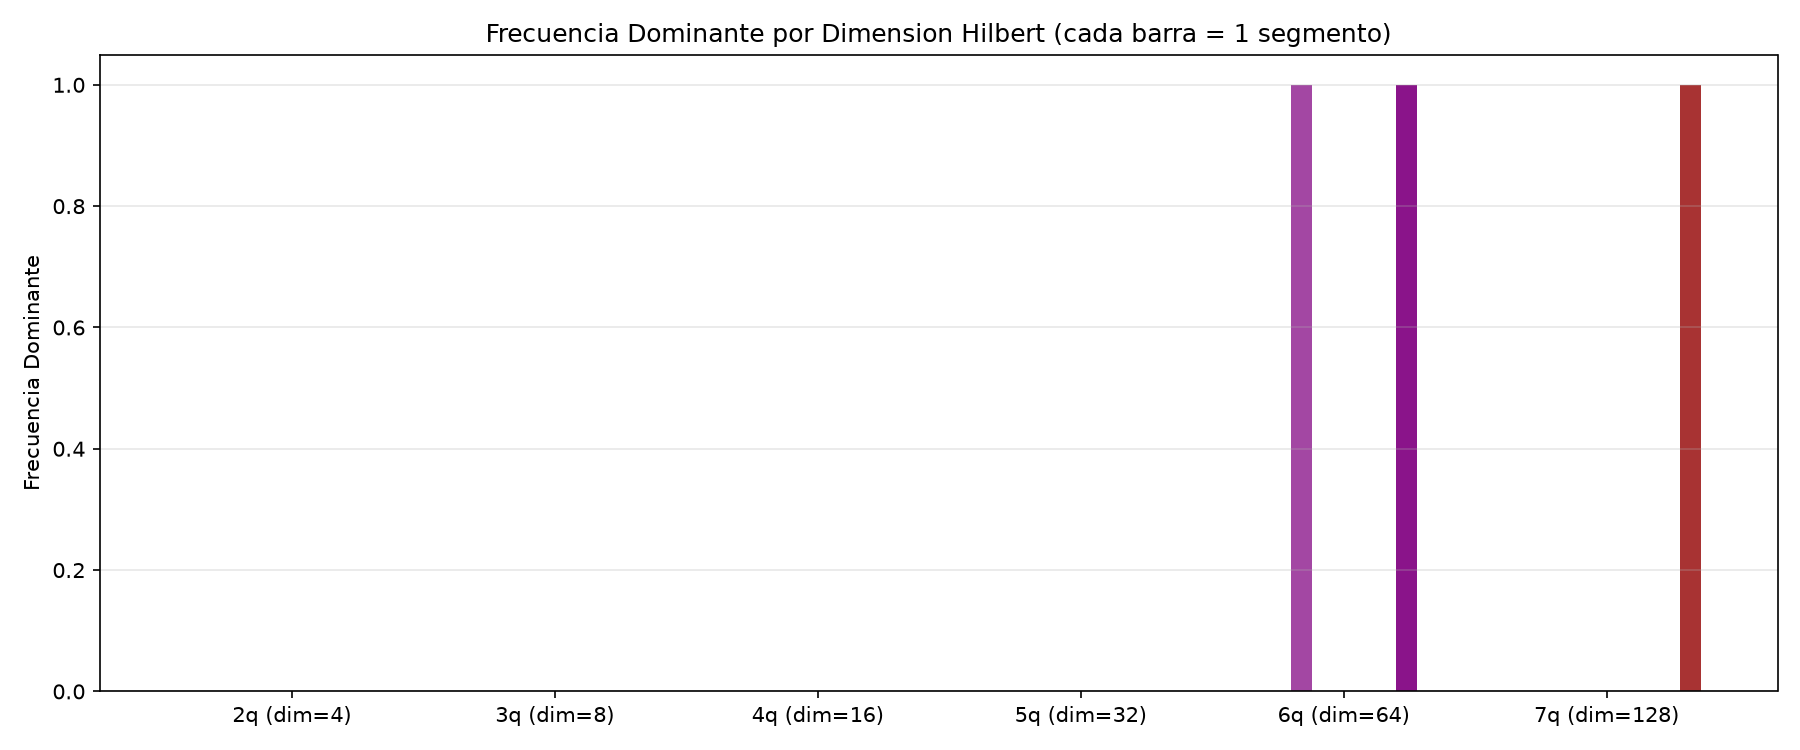
\includegraphics[width=\columnwidth]{frecuencia_dominante_por_dim.png}
\caption{Dominant frequency vs.\ Hilbert dimension. No consistent structure emerges across dimensions for amplitude encoding; frequencies fluctuate randomly, consistent with near-uniform states.}\label{fig:dom_freq}
\end{figure}

\begin{figure}[h]
\centering
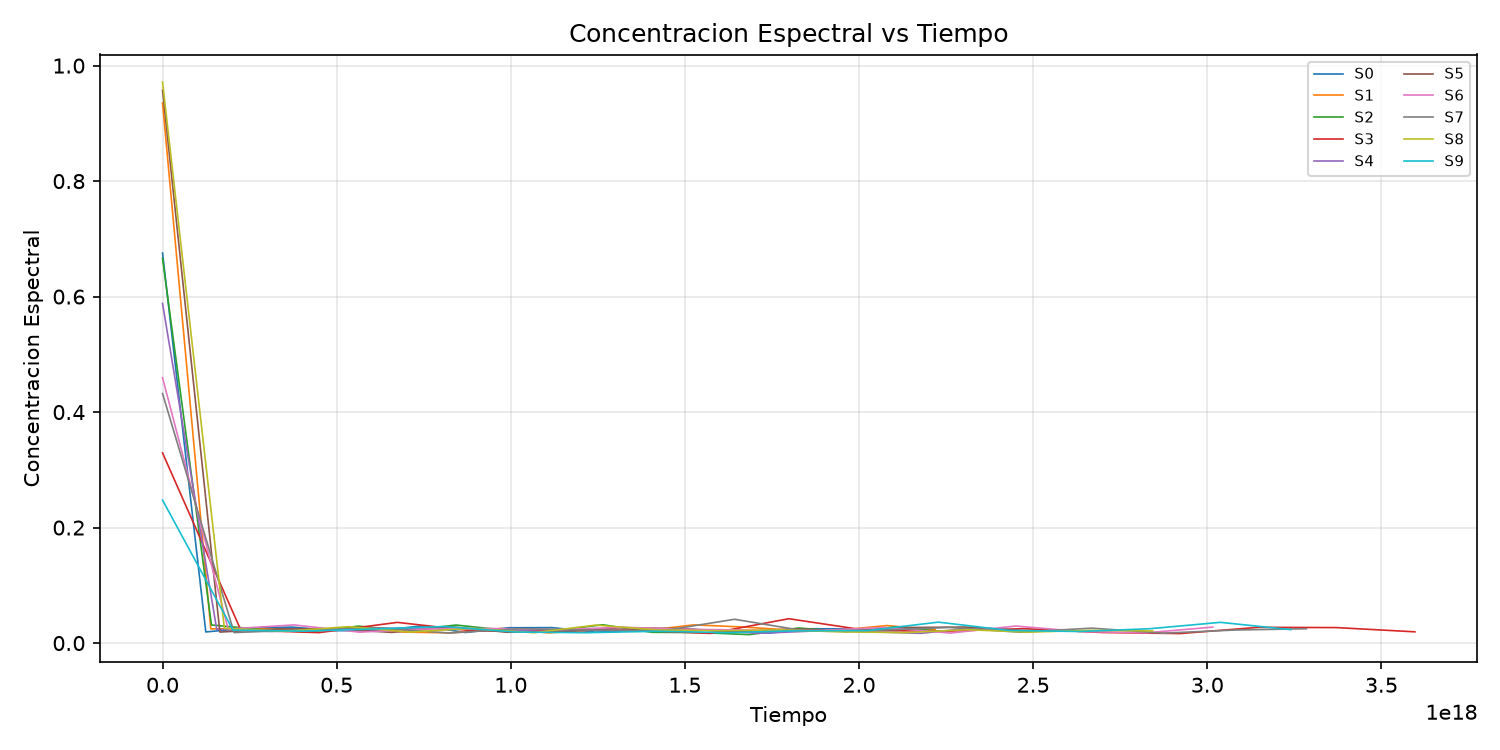
\includegraphics[width=\columnwidth]{concentracion_espectral.png}
\caption{Spectral concentration as a function of segment index and Hilbert dimension. Higher dimensions produce lower concentration, approaching the white noise limit.}\label{fig:spec_conc}
\end{figure}

\begin{figure}[h]
\centering
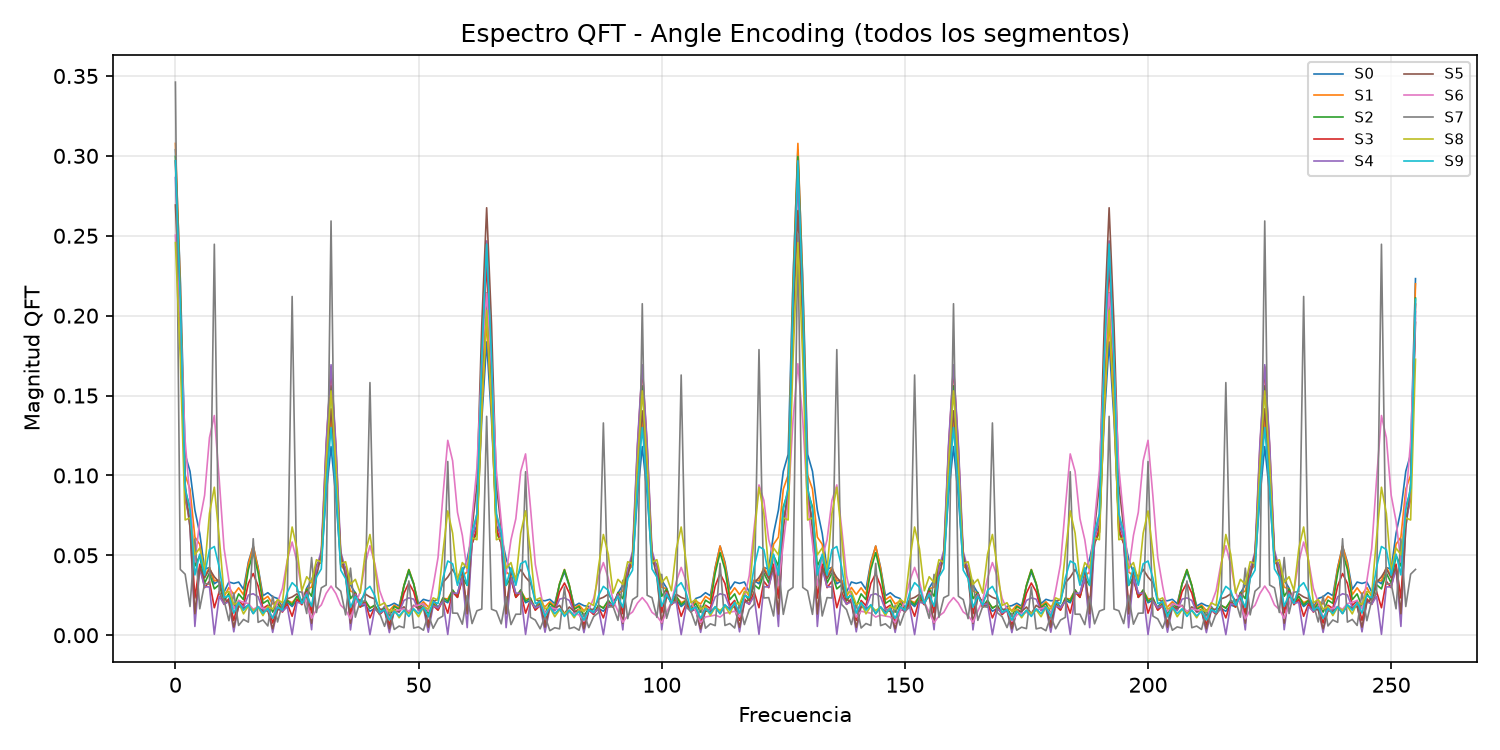
\includegraphics[width=\columnwidth]{angle_qft_all_segments.png}
\caption{Full QFT spectra for all angle-encoded segments. Unlike amplitude encoding, distinct spectral shapes emerge across segments, indicating that angle encoding preserves segment-specific structure.}\label{fig:angle_qft}
\end{figure}

\section*{Acknowledgments}

The author acknowledges the LIGO Scientific Collaboration and the Gravitational Wave Open Science Center for providing the O4b strain data. This research used Qiskit~\cite{qiskit2024} for quantum circuit simulation. AI-assisted language models were employed as an independent cross-validation agent for data analysis, equation derivation, and manuscript preparation (see Sec.~II-E); the author bears full responsibility for the content.

\begin{thebibliography}{00}

\bibitem{ligo2015}
J.~Aasi \textit{et al.} (LIGO Scientific Collaboration),
``Advanced LIGO,''
\textit{Class. Quantum Grav.}, vol.~32, no.~7, p.~074001, 2015.

\bibitem{verlinde2011}
E.~P.~Verlinde,
``On the Origin of Gravity and the Laws of Newton,''
\textit{J. High Energy Phys.}, vol.~2011, no.~4, p.~29, 2011.

\bibitem{hossenfelder2013}
S.~Hossenfelder,
``Minimal Length Scale Scenarios for Quantum Gravity,''
\textit{Living Rev. Relativity}, vol.~16, no.~1, p.~2, 2013.

\bibitem{schuld2018}
M.~Schuld and F.~Petruccione,
\textit{Supervised Learning with Quantum Computers}. Springer, 2018.

\bibitem{havlivcek2019}
V.~Havli\v{c}ek \textit{et al.},
``Supervised learning with quantum-enhanced feature spaces,''
\textit{Nature}, vol.~567, no.~7747, pp.~209--212, 2019.

\bibitem{gwosc}
Gravitational Wave Open Science Center,
\url{https://gwosc.org/}

\bibitem{qiskit2024}
IBM Quantum,
``Qiskit: An Open-Source Framework for Quantum Computing,''
\url{https://qiskit.org/}, 2024.

\bibitem{willsch2020}
D.~Willsch \textit{et al.},
``Benchmarking the quantum chip Q System One in the cloud,''
arXiv:2001.10611, 2020.

\end{thebibliography}

\end{document}
